\chapter*{\centering\large{2. Разработка программно-имитационной модели системы связи}}
\addcontentsline{toc}{chapter}{2. Разработка программно-имитационной модели системы связи}
\label{sec:Chapter2} \index{Chapter2}


	
	
\section*{\large{2.1 Разработка модели системы ретрансляции}}
\addcontentsline{toc}{section}{2.1 Разработка модели системы ретрансляции}
\begin{onehalfspace}

Система ретрансляции предполагает такой формат связи, что основные потребители, то есть абоненты, не находятся в прямой видимости антенн друг друга. В целом, две радиостанции могут обмениваться информацией на небольших расстояниях. Однако для увеличения зоны покрытия используются ретрансляторы, находящихся в прямой видимости антенн потребителей.

Примером ретрансляционной системы является набор из трёх радиостанций, две из них являются потребителями, а одна берёт на себя роль ретранслятора. Таким образом, разработка программно-имитационной модели системы связи включает в себя создание модели, состоящей из трёх радиостанций разного назначения. 

Такая модель может быть использована, к примеру, для оценки времени передачи информации между потребителями. При разработке модели системы передачи данных в канале радиосвязи можно выявить следующие факторы, влияющие на задержку времени и качество передачи:

\begin{enumerate} 

\item Расстояние, которое при известной скорости распространения (скорости света) является величиной пропорциональной времени задержки.

\item Время, затрачиваемое на кодирование, модуляцию, передачу, декодирование и обработку сигнала.

\item Затухание сигнала, по мере распространения сигнала через пространство он сталкивается с различными препятствиями, такими как здания, деревья, горы и другие преграды. Эти препятствия могут вызывать затухание, что может привести к уменьшению амплитуды сигнала.

\item В системах радиосвязи сигналы могут подвергаться помехам от других источников, эти помехи могут вызывать искажения сигнала. Искажения и помехи уменьшают вероятность корректной передачи данных.

\end{enumerate} 

Также на время передачи сигнала влияет пропускная способность канала. Если канал связи имеет ограниченную пропускную способность, то это может привести к потерям передачи. Реальные задержки могут зависеть от конкретных условий окружающей среды, используемого оборудования и других технических факторов.

При моделировании пропускной способности канала в системе одновременного приёма и передачи с двумя потребителями, процесса моделирования должен проводиться с учетом следующих факторов:

\begin{enumerate} 
\item Характеристики канала: Сначала необходимо определить характеристики канала, которые могут включать в себя пропускную способность, задержку, уровень шума и потери сигнала. Эти параметры могут быть получены из физических измерений или основаны на предыдущих исследованиях и моделях.

\item Модель передачи данных: Для моделирования передачи данных через канал можно использовать различные подходы, включая аналитические модели и симуляционные методы. Симуляция включает создание модели канала и передачи данных в программном окружении. Это позволяет анализировать поведение системы в различных условиях и изменять параметры канала, чтобы оценить их влияние на пропускную способность.

\item Анализ производительности: После моделирования и симуляции можно провести анализ производительности системы. Это может включать оценку пропускной способности канала, задержки передачи, потерь пакетов и других показателей производительности. Пропускная способность канала может быть измерена как количество переданных битов или пакетов данных в единицу времени. Анализ пропускной способности позволяет оценить, насколько эффективно канал используется для передачи данных. 
\end{enumerate} 

Моделирование задержек передачи данных в радиоканалах является важным аспектом проектирования и анализа систем связи. При моделировании задержек передачи данных в радиоканалах можно использовать различные подходы в зависимости от конкретной задачи и уровня детализации, необходимого для моделирования. Некоторые из распространенных подходов включают в себя:

\begin{enumerate} 
\item Аналитические модели: Для простых случаев и идеализированных условий можно использовать аналитические модели, основанные на математических выражениях и формулах. Например, моделирование задержек в прямой видимости может быть выполнено с использованием простых формул, учитывающих расстояние и скорость передачи данных.

\item Статистические модели: В случаях, когда задержки не могут быть точно предсказаны, можно использовать статистические модели, которые учитывают вероятностное распределение задержек. Это может быть особенно полезно при моделировании многолучевого распространения сигнала и влияния множества отражений и пути распространения сигнала.

\item Моделирование канала: Более сложные модели задержек могут быть получены с использованием моделей канала, которые учитывают различные характеристики радиоканала, такие как потери сигнала, задержки многолучевого распространения, шумы и искажения. 

\item Симуляции: Симуляции радиоканалов позволяют более точно моделировать задержки передачи данных, учитывая сложные факторы, такие как многолучевое распространение сигнала, интерференцию, эффекты перемещения объектов и другие. С помощью программных инструментов, таких как Matlab+Simulink можно создавать детальные модели.
\end{enumerate}     

	Для анализа погрешности была разработана модель временных задержек канала связи, включающая процессы приёма и передачи данных, обработки данных согласно протоколам связи, учитывающая скорость передачи данных, время распространения сигнала в среде и вычислительную мощность процессора. Модель задержек в канале связи приведена на рисунке 4. Рассматриваемая система описывает процесс передачи данных посредством радиосвязи в канале связи <<базовая станция — абонент>>, с помощью повторения сигнала на ретрансляторе. Подобная модель применима к реальной жизни, к примеру, описываемая систем позволяет описывать связь и передачу информационных сообщений на высокой скорости на дальние расстояния. 

\end{onehalfspace}

  \begin{center}
		\begin{figure}[h]
			\centering
			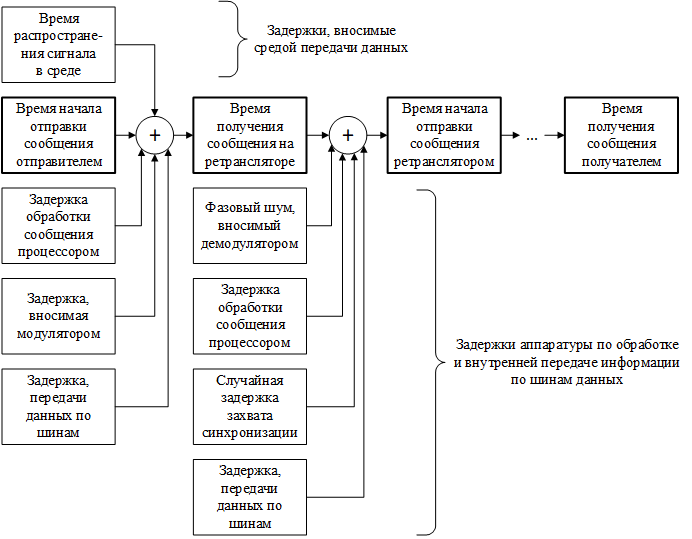
\includegraphics[width=1\linewidth]{sch1.png}
			\caption{Формирование модели временных задержек}
			\label{fig:model1}
		\end{figure}
	\end{center}

\begin{onehalfspace}

 
	Несмотря на ограничения по скоростям, пропускной способности и наличие временных задержек, ретрансляторы позволяю реализовывать устойчивые каналы связи с явно недоступными абонентами. Однако при моделировании процесса приёма и передачи, нужно обратить внимание на модель канала связи, которая будет использоваться. Часто в дополнение к шуму в модели канала связи учитывать и такие факторы как нестационарность каналов передачи, погрешности синхронизации (фазовой, частотной). Однако, если задача решается для дециметровых и сантиметровых диапазонов, уровень индустриальных и атмосферных помех радиоприема является низкий. Главный недостаток – ограниченное расстояние передачи и высокая степень зависимости от коммуникационной инфраструктуры – сети ретрансляторов. В таком случае важна максимальная дальность и скорость передачи данных. Таким образом, разработанная модель системы связи можно разделить на следующие логические части:

 \begin{enumerate} 

\item Модель канала позволяет анализировать влияние таких эффектов, как затухание, шум и другие искажения, на передачу и прием сигнала.

\item Модель приемника и передатчика, симулирующая процесс передачи сигнала, включая модуляцию и демодуляцию, кодирование и декодирование, фильтрацию и другие операции, выполняемые в блоке.  Модель позволяет изучать влияние различных параметров и алгоритмов передатчика на качество передачи сигнала в реальном времени.


\item Модель протоколов: Моделирует протоколы связи и алгоритмы, используемые для управления передачей данных и обеспечения надежности связи. Это включает в себя управление мощностью, управление доступом к каналу, коррекцию ошибок и другие функции протоколов.
\end{enumerate} 



  Разработанная модель состоит из трёх блоков:

 
	\begin{enumerate} 	
		\item БС — базовая станция, радиостанция, являющаяся потребителем; 
		
		\item Р — ретранслятор;
		
		\item А — абонент, радиостанция, являющаяся потребителем.
	\end{enumerate}
 
	Таким образом, модель представляет процесс передачи информации (пакета сообщения) в каналах <<базовая станция — ретранслятор>> и <<абонент — ретранслятор>>. В модель заложена возможность одновременного приёма и передачи информации (пакета сообщения) в канале <<базовая — абонент>>, система одновременного приёма и передачи внутри канала работает на разных частотах, что означает возможность одновременной двусторонней связи. Потребители могут одновременно отправлять и получать информацию без ожидания очереди. Для обеспечения более эффективной связи и уменьшения влияния сигнала передачи на сигнал приема, в системах одновременного приёма и передачи часто используются различные уровни мощности. Также модель ретранслятора должна удовлетворять следующему условию: в случае одновременного приёма ретранслятор принимает оба сообщения, после чего проверяет для установки получателя, после чего отправляет пакет на нужный адрес. Рисунок 5 демонстрирует описанный выше процесс передачи информации от удалённого оператора, который может быть представлен, как базовая станция, до абонента с помощью ретранслятора.  	

\end{onehalfspace}
    
	
	\begin{center}
		\begin{figure}[h]
			\centering
			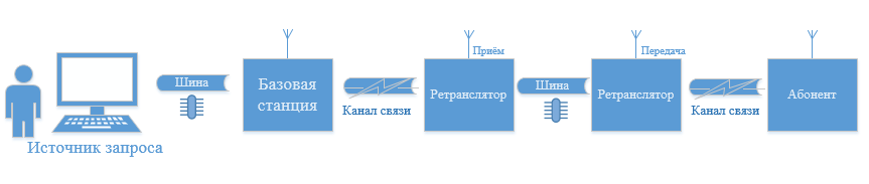
\includegraphics[width=1\linewidth]{ris1.png}
			\caption{Описание процесса}
			\label{fig:model6}
		\end{figure}
	\end{center}

 
\begin{onehalfspace}

	\begin{enumerate} 
	\item Удалённый пользователь формирует запрос к абоненту;
	\item Передача запроса на базовую станцию по шине данных;
	\item Передача кадра данных по радиосвязи;
	\item Приём кадра на ретрансляторе, обработка и маршрутизация, передача кадра по радиосвязи;
	\item Приём кадра и обработка запроса абонентом.
	\end{enumerate} 

 На рисунке 6 демонстрируется структурная схема модели «базовая станция – ретранслятор – абонент», включающая в себя физические блоки обмена информацией, такие как блоки приёма/передачи и обработки сигнала.
 
 \begin{figure}[H]
			\centering
			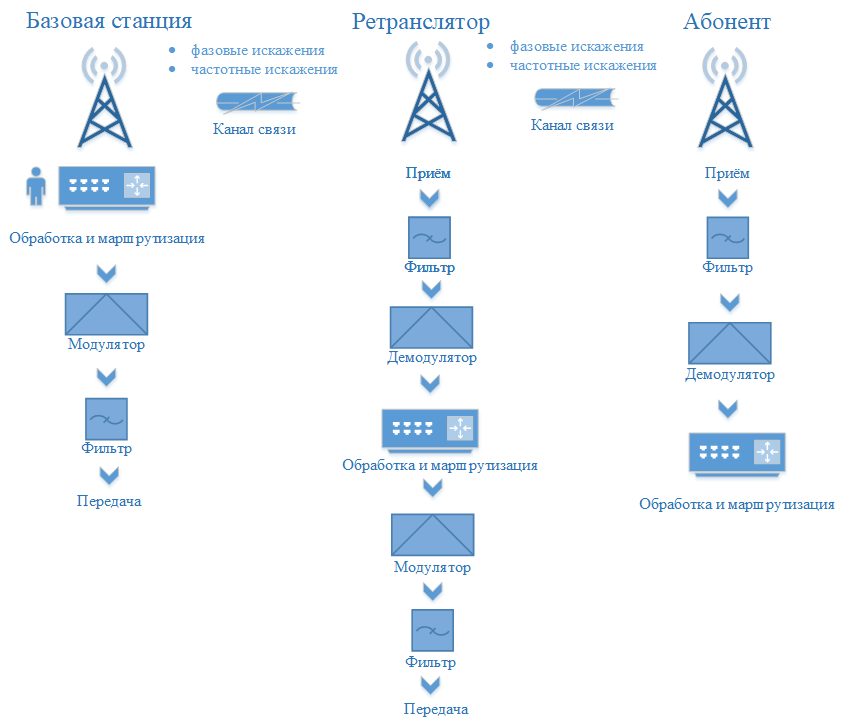
\includegraphics[width=1\linewidth]{struct_retr.png}
			\caption{Структурная схема процесса}
			\label{fig:model7}
	\end{figure}


 Модель радиосвязи может быть применена для анализа и симуляции процессов обмена данными между удалёнными потребителями в режиме реального времени, к примеру, для тестирования и отработки алгоритмов связи, с целью проверки реальных изделий. Программным обеспечением, позволяющим моделировать в реальном времени является, к примеру, используемый в работе Matlab+Simulink. Режим реального времени является режимом обработки данных, при котором обеспечивается взаимодействие вычислительной системы с внешними по отношению к ней процессами в темпе, соизмеримом со скоростью протекания этих процессов. Такие модели позволяют изучать и оценивать работу радиосвязи в реальных условиях и в реальном времени, что особенно важно при разработке и тестировании радиосистем.
 
В реальном времени задержка становится критическим фактором. Подобные модели радиосвязи должны быть спроектированы таким образом, чтобы минимизировать задержку передачи и обработки сигнала. Вычислительная эффективность, включающая оптимизацию алгоритмов и структур данных, выбор эффективных алгоритмов обработки данных является способом уменьшения времени задержки передачи данных, это также должно быть учтено в части модели, отвечающей за протоколы. 

Минимизация модельной задержки требует использования оптимизированных алгоритмов обработки сигнала, параллельной обработки и оптимизации пропускной способности системы. Оптимизация и эффективная организация обработки сигнала, определяет возможность модели подстраиваться под различные эксперименты, а также переиспользоваться с учётом даже критических изменений в сигнале и протоколах связи.


Модели радиосвязи требуют тщательного тестирования и верификации для обеспечения их правильной работы в реальном времени. Это может включать сравнение результатов моделирования с реальными измерениями и оценку соответствия критериям производительности и качества. 


На основе описанных выше принципов была построена расширенная модель канала связи <<базовая станция — ретранслятор — абонент>>, которая состоит из модели канала, моделей приёмников и передатчиков, моделей обработчиков, полученных сообщений. Каждая из моделей оказывает влияние на итоговую временную задержку времени передачи сигнала. К примеру, временные задержки появляются и здесь, в связи с синхронизацией пакетов данных, проверкой целостности пакетов и передачей данных на физическом уровне, зависящей от среды передачи. Также для построение модели временных задержек передачи данных в канале радиосвязи с ретранслятором проведён системный анализ факторов, влияющих на точность программно-имитационного моделирования. 


Данные в канале <<базовая станция — абонент>> подвергаются следующим манипуляциям:

	\begin{enumerate} 
		\item Обработка данных внутри ретранслятора и абонента — декодировка и демодуляция, а также преобразование в форму понятную соответствующему потребителю.
	    \item Передача данных внутри канала радиосвязи — формирование сигнала, выделение несущей частоты, модуляция.
	\end{enumerate} 
 
Модель даёт оценку временных задержек ping-сигнала в канале <<базовая станция — абонент>>. В данном случае, информацией в радиоканале является ping-сигнал. Базовая станция формирует запрос к абоненту, передаёт сообщение на ретранслятор, находясь в режиме ожидания ответа от абонента. Ретранслятор, получив пакет от базовой станции, обрабатывает его внутри согласно логике своего внутреннего протокола работы, и отправляет сообщение в соответствующий канал (в данном случае, канал радиосвязи <<ретранслятор — абонент>>). Абонент, приняв сообщение, отправляет ответ о его получении на ретранслятор, после распаковывает его и отрабатывает согласно командам, полученным в сообщении от базовой станции. Ретранслятор, получив пакет от абонента, маршрутизирует его внутри согласно логики его внутреннего роутера, и отправляет сообщение в соответствующий канал (в данном случае, канал радиосвязи <<ретранслятор — базовая станция>>) и переходит в режим ожидания. На рисунке 7 кратко показана логика построения модели обработки полученной из сигнала информации, так из-за работы со сложными структурами данных время может тратиться на их обработку.


\end{onehalfspace}
 
	\begin{center}
		\begin{figure}[h!]
			\centering
			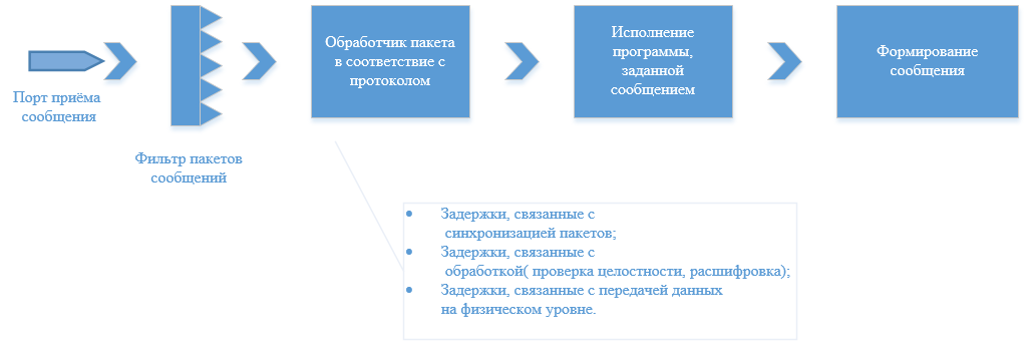
\includegraphics[width=1\linewidth]{ris3.png}
			\caption{Моделирование обработки информации}
			\label{fig:model8}
		\end{figure}
	\end{center}

	\begin{onehalfspace}
	Согласно схеме на рисунке 1 модель классифицируется по четырём параметрам: 
	\begin{enumerate} 
		\item По отношению к применимости физической модели – рассматривается ситуация передачи сигнала посредством радиосвязи от источника к явно недоступному, не в зоне видимости, потребителю. Для повторения и передачи сигнала используется ретранслятор. Подобная модель применима к реальной жизни, к примеру, позволяет исследовать связь на высокой скорости на большом расстоянии, в итоговую задержку закладывается время распространения сигнала в среде.
		\item По отношению к применимости математической модели – модели системы передачи данных с помощью радиосвязи, основываются на математических выражениях, которые описывают характеристики канала и передаваемые сигналы. Условия наличия гауссовского шума в канале, а также граничные условия на уравнения распространения радиоволн, соответствующего диапазона, определяет возможность получения аналитического решения.
		\item По отношению к мощности вычислительной базы – запуск модели производился на компьютере, с известными производительностью и тактовой частотой.
		\item По отношению ко времени – модельная шкала времени соответствует реальному времени.
   \end{enumerate}
	
			
	 На рисунке 8 демонстрируется имитационная модель системы «базовая станция – ретранслятор – абонент» в Simulink, учитывающая процессы модуляции, демодуляции и фильтрации сигнала. 
\end{onehalfspace}
 
 \begin{center}
		\begin{figure}[h!]
			\centering
			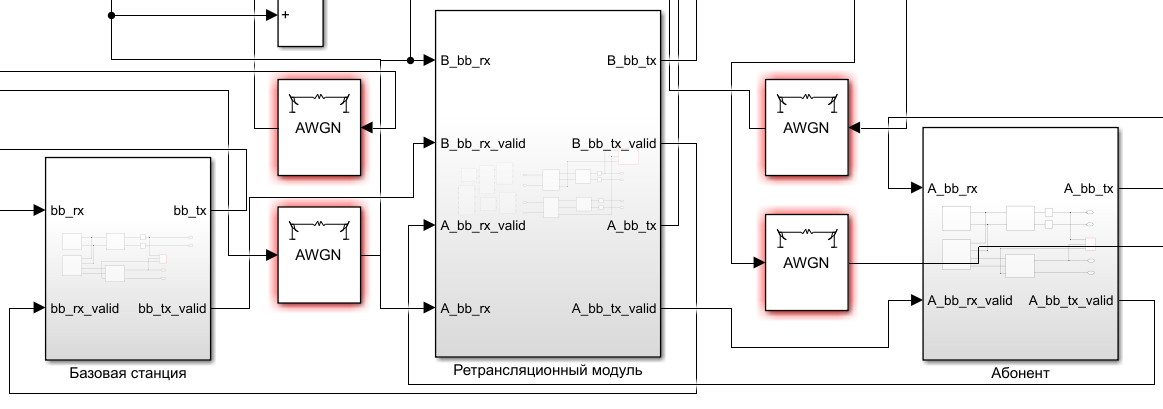
\includegraphics[width=1\linewidth]{bigger1.png}
			\caption{Модель системы связи «базовая станция – ретранслятор – абонент»}
			\label{fig:model9}
		\end{figure}
	\end{center}

	
\begin{onehalfspace}	
	
	 В основе каждого из блоков БС, Р, А лежат блоки приёма $RX$ и передачи $TX$. Блок передачи ($TX$ на схемах) состоит из входа сообщения, которое необходимо подготовить к отправке потребителю. Сообщение, обрабатывается в соответствие с протоколом данного типа сообщений. Информация может быть представлена битовом виде далее кодированное сообщение изменяется модулятором, далее для сохранения полезной информации о сигнале, сообщение, проходит через фильтр и попадает в передающий канал.

  На рисунке 9 показаны имитационные модели блоков приёма и передачи в Simulink. Блок приёма ($RX$ на схемах) состоит из входа сообщения, которое пришло от какого-либо из потребителей, сигнал проходит ответный к $TX$ фильтр, также подвергается процедуре демодуляции, принятая информация может быть представлена битовом виде, далее декодированное сообщение передаётся на блок логики обработки принятых сообщений.

  Однако вместе с основным передаваемым информационным радиосигналом на приемник $RX$ воздействуют и помехи различной природы, что вызывает различное искажение принятой информации.

\end{onehalfspace}	


\begin{center}
		\begin{figure}[h!]
			\centering
			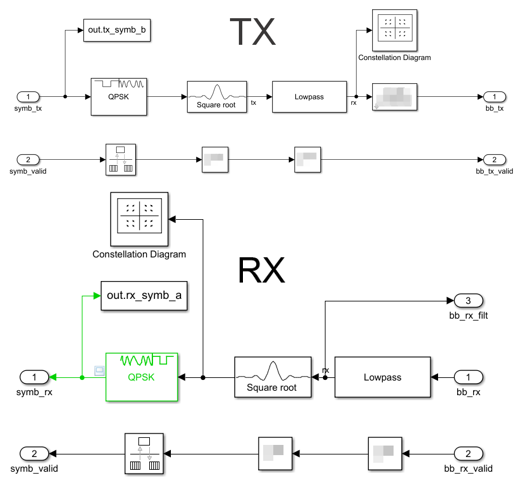
\includegraphics[width=1\linewidth]{bigger2.png}
			\caption{Модель блоков приёма и передачи. Блок передачи ($TX$ на схемах) и  Блок приёма ($RX$ на схемах)}
			\label{fig:model9}
		\end{figure}
	\end{center}





\begin{onehalfspace}
	
	 В модели рассматривается влияние на качество принятой информации и время её приёма, в канале <<базовая станция — абонент>>, атмосферных шумов и задержек, возникающих из-за внутренних процессов каждого из модулей базовая станция, ретранслятор и абонент. Для установления связи между модулями на приёмные и передающие частоты накладываются следующие условия:
    
	
	\begin{center}
	$\nu_{b_{tx}} = \nu_{rtb_{rx}},$
	 
	где $\nu_{b_{tx}}$ — передающая частота базовой станции, $\nu_{rtb_{rx}}$ — приёмная частота ретранслятора.
	 
	 
	$\nu_{b_{rx}} = \nu_{rtb_{tx}},$
	 
	где $\nu_{b_{rx}}$ — приёмная частота базовой станции, $ \nu_{rtb_{tx}}$ — передающая частота ретранслятора.
	\end{center}
	 
	 
	\begin{center}
	$\nu_{rta_{tx}} = \nu_{a_{rx}},$
	 
	где $\nu_{rta_{tx}} $ — передающая частота ретранслятора, $\nu_{a_{rx}}$ — приёмная частота абонента.
	 
	 
	$\nu_{rta_{rx}} = \nu_{a_{tx}},$
	 
	где $\nu_{rta_{rx}} $ — приёмная частота ретранслятора, $\nu_{a_{tx}}$ — передающая частота абонента.
	\end{center}

	
	Также шумы и помехи складываются с сигналом. Таким образом модель является имитацией канала связи с шумом.	Шум модели представляется моделью аддитивного белого гауссовского шума (АБГШ).

\end{onehalfspace}
 
	\begin{center}
		\begin{figure}[h!]
			\centering
			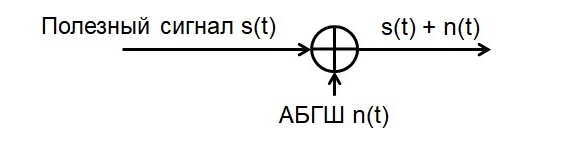
\includegraphics[width=0.55\linewidth]{shum.jpg}
			\caption{Модель канала с шумом}
			\label{fig:model11}
		\end{figure}
	\end{center}

 
\begin{onehalfspace}
Конечность скорости распространения радиосигнала, как электромагнитной волны, в среде также влияет на время приёма сигнала, в частности это даёт неопределённость в расчёте начальной фазы сигнала. Также модель учитывает фактор замирания сигнала, то есть накладывание собственных копий сигнала от переотражений с разными фазами. Это существенный фактор, вызывающий задержки обработки на ретрансляторе, поддерживающим режим одновременных приёма и передачи.
\end{onehalfspace}
	
	\newpage
	\pagebreak
	\clearpage
	
	\section*{\large{2.2 Структура модели базовой станции}}
    \addcontentsline{toc}{section}{2.2 Структура модели базовой станции}
\begin{onehalfspace}

В разработанной модели базовая станция имеет один канал связи с ретранслятором. Базовая станция может работать со следующими типами сигналов: 
		\begin{enumerate} 	
		\item Сигнал, являющийся сообщением для ретранслятора. 
	
		\item Сигнал, являющийся сообщением для абонента.

            \item Сигнал, являющийся сообщением, полученным от абонента. 
	
		\item Сигнал, являющийся сообщением, полученным от ретранслятора.
	\end{enumerate}

	На рисунке 11 представлен блок схема базовой станции, состоящая из следующих блоков: 
	
	\begin{enumerate} 	
		\item $Data \ Generator$ блок, отвечающий за формирование пакета сообщения к потребителю, создаёт строку-сообщение, которая обрабатывается в соответствие с протоколом обработки данных сообщений (к примеру, добавляет заголовок сообщения), приводит к битовому виду. 
		
		\item  $Data \ Verification$ блок отвечающий за проверку данных. В частности, в случае отработки сценария ping базовая станция — абонент, проверяет соответствие ответного пакета от абонента и пакета-запроса от базовой станции.
		
		\item  $RX$ описание приведено в 2.1 Разработка модели системы ретрансляции.
		
		\item  $TX$ описане приведено в 2.1 Разработка модели системы ретрансляции.
	\end{enumerate}
	
    Модель имеет следующие входы и выходы информации: 
    \begin{enumerate} 	
		\item $bb\_rx$ — вход для полезного сигнала принятого с ретранслятора, моделирует часть физического канала передачи.
  
            \item $bb\_rx\_valid$ — вход для вспомогательного сигнала валидности принятого с ретранслятора.

            \item $bb\_tx$ — выход для полезного сигнала передаваемого на ретранслятор, моделирует часть физического канала передачи.
  
            \item $bb\_tx\_valid$ — выход для вспомогательного сигнала валидности передаваемого на ретранслятор.
\end{enumerate}


\begin{center}
		\begin{figure}[h!]
			\centering
			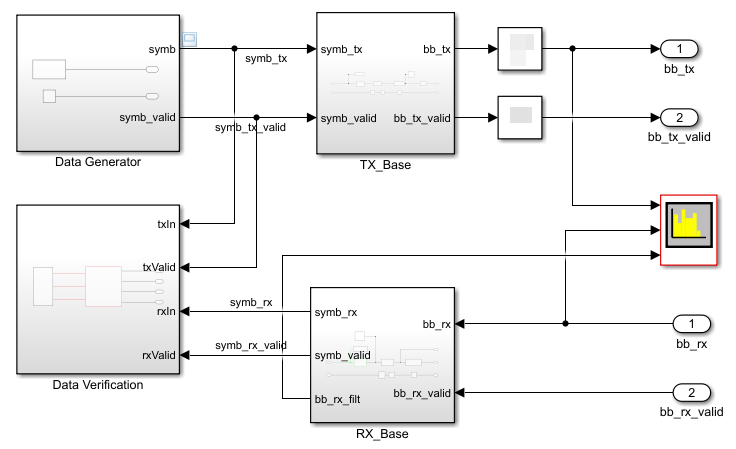
\includegraphics[width=1\linewidth]{bigger3.png}
			\caption{Модель базовой станции}
			\label{fig:model12}
		\end{figure}
	\end{center}

Сообщение, сформированное базовой станцией в блоке $Data \ Generator$ попадает на блок $TX$, где подвергается трансформации в пригодную форму для передачи по каналу, далее он передаётся на выход $bb\_tx$. Сигнал, принятый базовой станцией со входа $bb\_rx$ попадает на блок $RX$, в котором осуществляется конвертация его в выбранную для дальнейшей обработки форму. К примеру, в случае моделируемого процесса приёма и передачи ping-сигнала в канале <<базовая станция — абонент>>, полученный набор символов, после демодуляции в блоке $RX$, переводится в битовую последовательность в блоке $Data \ Verification$ и преобразовывается в число, которое сравнивается с числом, которое ожидается получить от ретранслятора или абонента. Далее если полученное сообщение соответствует сообщению ожидаемому от абонента, то ping считается успешным.

	
	
\end{onehalfspace}




\section*{\large{2.3 Структура модели ретранслятора}}
 \addcontentsline{toc}{section}{2.3 Структура модели ретранслятора}
 
\begin{onehalfspace}


В разработанной модели ретранслятор имеет два канала связи. Прямой канал с абонентом и прямой канал с базовой станцией. Ретранслятор может обрабатывать следующие сигналы: 


\begin{enumerate} 	
	\item Сигнал, являющийся сообщением для абонента.

        \item Сигнал, являющийся сообщением, полученным от абонента.

        \item Сигнал, являющийся сообщением для базовой станции.

        \item Сигнал, являющийся сообщением, полученным от базовой станции.
\end{enumerate}


На рисунке 12 представлен блок схема ретранслятора, состоящая из: 

\begin{enumerate} 	
	\item $RX\_FromAbo$ блок приёма сигнала абонента, содержащий в себе блок $RX$, описание которого приведено в описание приведено в 2.1 Разработка модели системы ретрансляции, а также блоки \\ $Data \ Verification \ Base$, $Data \ Verification \ Abo$ аналогичные описанным в 2.2 Структура модели базовой станции. 
	
	\item  $RX\_FromBase$ аналогично блоку $RX\_FromAbo$.
	
	\item  $TX\_ToAbo$ блок передачи сигнала абоненту, содержащий в себе блок $TX$, описание которого приведено в описание приведено в 2.1 Разработка модели системы ретрансляции, а также блоки \\ $Data \  Generator \ Base$, $Data \  Generator \ Abo$ аналогичные описанным в 2.2 Структура модели базовой станции.

        \item  $TX\_ToBase$ аналогично блоку $RX\_FromBase$.
        
\end{enumerate}
\end{onehalfspace}


 Модель имеет следующие входы и выходы информации: 
    \begin{enumerate} 	
		\item $A\_bb\_rx$ — вход для полезного сигнала принятого от абонента, моделирует часть физического канала передачи.

            \item $B\_bb\_rx$ — вход для полезного сигнала принятого от базовой станции, моделирует часть физического канала передачи.
  
            \item $A\_bb\_rx\_valid$ — вход для вспомогательного сигнала валидности принятого от абонента.

            \item $B\_bb\_rx\_valid$ — вход для вспомогательного сигнала валидности принятого от базовой станции.

            \item $A\_bb\_tx$ — выход для полезного сигнала передаваемого абоненту, моделирует часть физического канала передачи.

             \item $B\_bb\_tx$ — выход для полезного сигнала передаваемого базовой станции, моделирует часть физического канала передачи.
  
            \item $A\_bb\_tx\_valid$ — выход для вспомогательного сигнала валидности передаваемого абоненту.

             \item $B\_bb\_tx\_valid$ — выход для вспомогательного сигнала валидности передаваемого базовой станции.
\end{enumerate}

\begin{figure}[h!]
	\centering
	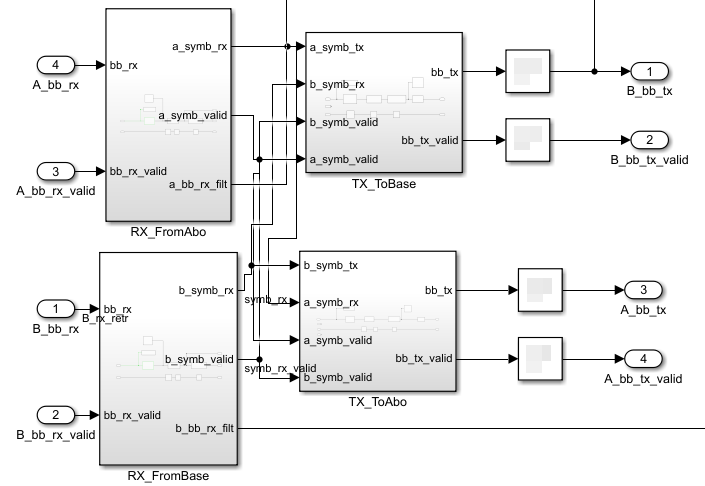
\includegraphics[width=1\linewidth]{bigger4.png}
	\caption{Модель ретранслятора}
	\label{fig:model14}
\end{figure}

Сигнал, полученный от какого-либо из потребителей приходит на соответствующий информационный вход $B\_bb\_rx$ или $A\_bb\_rx$. Далее, сигнал попадает на соответствующий блок приёма, например, $RX\_FromBase$, где преобразовывается в удобный для обработки вид. Если полученное сообщение оказалось ожидаемым ping-сигналом от базовой станции к абоненту, то оно попадает в блок $TX\_ToAbo$, после чего передаётся на выход $A\_bb\_tx$.



\begin{figure}[h!]
		\centering
		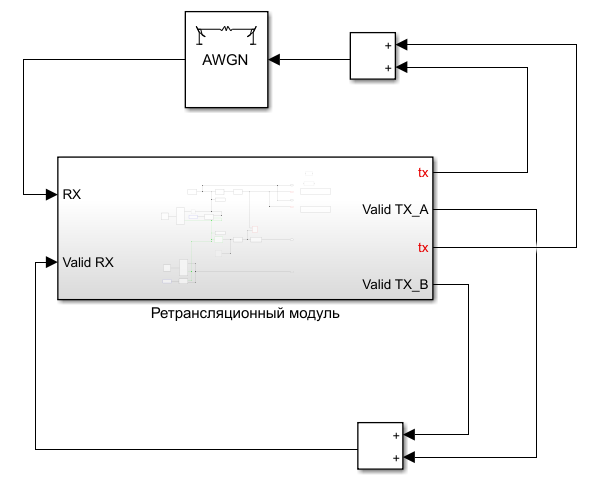
\includegraphics[width=0.5\linewidth]{retr1.png}
		\caption{Модель ретрансляцинного модуля, внешняя часть}
		\label{fig:model15}
	\end{figure}



\section*{\large{2.4 Структура модели абонента}}
 \addcontentsline{toc}{section}{2.4 Структура модели абонента}

\begin{onehalfspace}

В разработанной модели абонент имеет один канал связи с ретранслятором. Абонент может работать со следующими типами сигналов: 
		\begin{enumerate} 	
		\item Сигнал, являющийся сообщением для ретранслятора. 
	
		\item Сигнал, являющийся сообщением для базовой станции.

	
		\item Сигнал, являющийся сообщением, полученным от ретранслятора.

            \item Сигнал, являющийся сообщением, полученным от базовой станции. 
            
	\end{enumerate}



На рисунке 14 представлен блок схема абонента, состоящая из следующих блоков: 

\begin{enumerate} 	
	\item $Data \ Generator$ блок, описание которого приведено в 2.2 Структура модели базовой станции; 
	
	\item  $Data \ Verification$ блок, описание которого приведено в 2.2 Структура модели базовой станции;
	
	\item  $RX$ блок, описание которого приведено в 2.1 Разработка модели системы ретрансляции.
	
	\item  $TX$ блок, описание которого приведено в 2.1 Разработка модели системы ретрансляции.
\end{enumerate}

Модель имеет следующие входы и выходы информации: 
    \begin{enumerate} 	
		\item $A\_bb\_rx$ — вход для полезного сигнала принятого с ретранслятора, моделирует часть физического канала передачи.
  
            \item $A\_bb\_rx\_valid$ — вход для вспомогательного сигнала валидности принятого с ретранслятора.

            \item $A\_bb\_tx$ — выход для полезного сигнала передаваемого на ретранслятор, моделирует часть физического канала передачи.
  
            \item $A\_bb\_tx\_valid$ — выход для вспомогательного сигнала валидности передаваемого на ретранслятор.
\end{enumerate}

\end{onehalfspace}

\begin{figure}[h!]
	\centering
	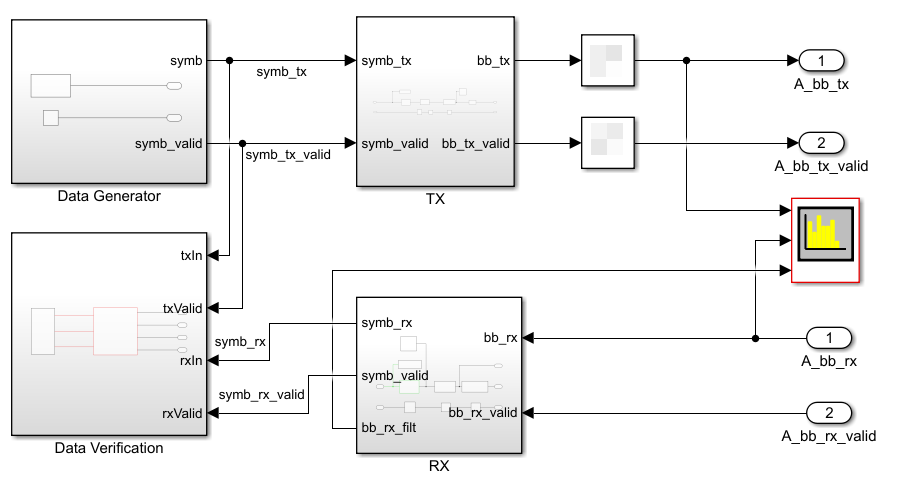
\includegraphics[width=1\linewidth]{bigger5.png}
	\caption{Модель абонента}
	\label{fig:model17}
\end{figure}


Сигнал, переданный ретранслятором, поступает на вход $A\_bb\_rx$. Далее он попадает в блок обработки принятого сигнала $RX$, после приведения его к понятному для следующего блока виду, он попадает в $Data \ Verification$, где происходить проверка того, является ли принятое от ретранслятора сообщение ping-сигналом от базовой станции. То оно попадает в блок $Data \ Generator$, формирующий ответной сообщение, далее, пройдя обработку в передающем блоке $TX$ попадает на выход $A\_bb\_tx$. 


\begin{figure}[h!]
	\centering
	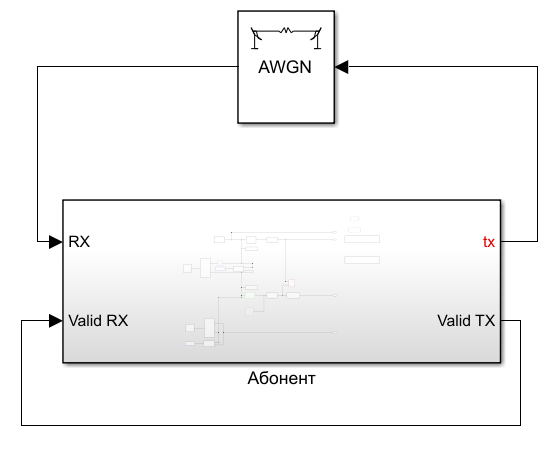
\includegraphics[width=0.5\linewidth]{abo1.png}
	\caption{Модель абонента, внешняя часть}
	\label{fig:model18}
\end{figure}


\newpage
\section*{\large{2.5 Описание принципа учёта задержек системы ретрансляции}}
 \addcontentsline{toc}{section}{2.5 Описание принципа учёта задержек системы ретрансляции}

\begin{onehalfspace}

Для расчёта модельных задержек времени передачи сигнала используются дополнительные линии передачи $Valid \ RX$ и $Valid \ TX$, которые идут параллельно соответствующему сигналу приёма или передачи:

\begin{enumerate} 	
	
	\item $bb\_tx\_valid - B\_bb\_rx\_valid$ — канал валидности <<базовая станция — ретранслятор>>  — для отработки задержек модуляции и логики обработки сообщения; 
	
	
	\item  $A\_bb\_tx\_valid - A\_bb\_rx\_valid$ — канал валидности <<ретранслятор — абонент>>  — для отработки задержек модуляции и логики обработки сообщения;
	
	\item  $bb\_tx\_valid - B\_bb\_rx\_valid - A\_bb\_tx\_valid - A_bb\_rx\_valid$ — канал валидности <<базовая станция — абонент>> — состоит из предыдущих двух пунктов предназначен для отработки задержек модуляции и логики обработки сообщения;
		
	\item  $A\_bb\_tx\_valid - A\_bb\_rx\_valid$ — канал валидности <<абонент — ретранслятор>>;
	
	\item  $B\_bb\_tx\_valid - bb\_rx\_valid$ — канал валидности <<ретранслятор — базовая станция>>;
	
	\item  $bb\_tx\_valid - B\_bb\_rx\_valid - A\_bb\_tx\_valid - A\_bb\_rx\_valid$ — канал валидности <<абонент — базовая станция>> —  состоит из предыдущих двух пунктов предназначен для отработки задержек модуляции и логики обработки сообщения;
	
	\item  $bb\_tx\_valid - bb\_rx\_valid$ — внутренний канал валидности <<базовая станция — базовая станция>> — для отработки задержек из-за собственного сигнала передачи;
	
	\item  $A\_bb\_tx\_valid - A\_bb\_rx\_valid$ — внутренний канал валидности <<абонент — абонент>>  — для отработки задержек из-за собственного сигнала передачи;
	
	\item  $B\_bb\_tx\_valid - B\_bb\_rx\_valid, A\_bb\_tx\_valid - A\_bb\_rx\_valid$ — внутренние каналы валидности ретранслятора — для отработки задержек из-за собственного сигнала передачи.



\end{enumerate}

Эти каналы валидности позволяют отследить насколько сигнал, пришедший в конкретный блок модулятора, фильтра или конвертации типа данных, отстаёт от сигнала сформированного передатчиком. Это линия идёт параллельно всем линиям приёма и передачи модели, что позволяет компенсировать модельные задержки и синхронизовать модельные приёмник и передатчик внутри каждого канала связи.
\end{onehalfspace}
